\thispagestyle{empty}

\section{Grundlagen der Virtualisierung}
\label{Grundlagen der Virtualisierung}
Es existieren verschiedenen Ansätze für Virtualisierung, wie zum Beispiel die in dieser Arbeit betrachtete Container- oder Hypervisor-basierte Virtualisierung. Die Virtualisierung wird verwendet, um Hardware effizienter zu nutzen. Dabei wird die Hardware virtuell in kleinere Einheiten zerlegt, die voneinander isoliert sind. Auf diesen Einheiten können Prozesse ausgeführt werden, die nichts von den Prozessen in anderen Einheiten wissen. Dabei ist vor allem die Isolierung dieser Einheiten von Interesse.

Dieses Kapitel beschäftigt sich zunächst mit dem Container-basierten Virtualisierungsansatz. Im Anschluss wird auf die Hypervisor-basierte Virtualisierung eingegangen. 

\subsection{Container-basierte Virtualisierung}
Container-basierte Virtualisierung ist ein leichtgewichtiger Virtualisierungsansatz auf Betriebssystemebene, bei dem das  Gastgeberbetriebssystem (Host) zur Ausführung mehrerer virtueller Umgebungen verwendet wird. Diese virtuellen Umgebungen werden oft einfach als \emph{Container} bezeichnet. \emph{Linux-V} \cite{Overview2018PaperLinux-VServer}, \emph{Open VZ} \cite{IndexOpenvz.org} und \ac{LXC} \cite{IndexLinuxcontainers.Org} sind die drei wichtigsten Vertreter dieses Virtualisierungsansatzes. In dieser Arbeit wird vor allem auf den Linux-Container (LXC) eingegangen. Dieser bildet die Grundlage der im praktischen Abschnitt verwendeten Softwarelösung \emph{Docker} \cite{MeineDockerPlatform}. 

In Abbildung \ref{fig:architecture} sind die allgemeinen Architekturen der beiden Virtualisierungsansätze, der Container-basierte und der Hypervisor-basierte, gegenübergestellt. Die Basis beider Techniken ist die Host-Hardware, im Bild als unterster Baustein \emph{Hardware} gezeigt. Im Folgenden wird nur die linke Seite \emph{container-based architecture} weiter betrachtet. Container-basierte Virtualisierung erfolgt, wie bereits erwähnt, auf Betriebssystemebene. Das bedeutet, dass Container neben anderen Anwendungen auf dem Host-System, ohne redundant ausgeführte Betriebssysteme laufen können. Im Bild wird dies durch den Baustein \emph{Shared Operating System} dargestellt, auf dem die Bausteine \emph{Container} aufbauen. 
Container stellen eine isolierte Umgebung mit den notwendigen Ressourcen für die Ausführung von Anwendungen (\emph{App}) dar. 

Ressourcen können entweder mit dem Host geteilt oder separat im Container installiert werden. Container sehen von außen aus wie normale Prozesse, die auf dem \emph{Kernel} laufen. Der Kernel ist der Kern eines Betriebssystems, der die Schnittstelle zur Hardware bildet und für die Ressourcenverwaltung verantwortlich ist. Der Betriebssystem-Kernel wird im Fall der Container-Virtualisierung mit den Containern geteilt. 

Die Basis der Linux-Container bilden die sogenannten \emph{Namespaces} \cite{Also2018Man7.orgMan-pages}. Diese stellen in Verbindung mit anderen Ressourcen-Management-Systemen eine isolierte Umgebung in Form dieser Container zur Verfügung. Der in dieser Arbeit betrachtete Virtualisierungsansatz LXC verwendet die Linux \emph{control group}-Ressourcenverwaltungseinrichtung als Grundlage \cite{Heo2015ControlV2} und fügt \ac{POSIX}\emph{-file capabilities} \cite{Overview2018PaperLinux-VServer} hinzu, um die Ressourcen der verschiedenen Container einzuschränken.



%Die allgemeine Architektur einer Container-basierten Virtualisierungs Lösung ist in Abbildung \ref{fig:architecture} dargestellt. Container basierte Virtualisierung erfolgt wie bereits erwähnt auf Betriebssystem Ebene. Das bedeutet, dass mehrere Anwendungen ohne redundante Ausführung anderer Betriebssysteme auf dem Host betrieben werden können. Container sehen von außen aus wie normale Prozesse, die auf dem Kernel laufen, der mit dem Host-Rechner geteilt wird. Der Kernel ist so zu sagen der Kern eines Betriebssystems, der die Schnittstelle zur Hardware bildet und für die Ressourcenverwaltung grundverantwortlich ist. Container stellen eine isolierte Umgebung mit den notwendigen Ressourcen für die Ausführung von Anwendungen dar. Diese Ressourcen können entweder mit dem Host geteilt oder separat im Container installiert werden \cite{Xavier2014AClusters}. Namespaces sind die Basis des Linux-Container und stellen in Verbindung mit anderen Ressourcen-Management-Systemen eine isolierte Umgebung in Form von Containern zu Verfügung. LXC nimmt die Linux Cgroup (Controll Group) Ressourcenverwaltungseinrichtungen\cite{Heo2015ControlV2} als Grundlage und fügt POSIX file Capabilities\cite{Overview2018PaperLinux-VServer} hinzu, um die Ressourcen unter den Containern einzuschränken. 




\vspace{1em}
\begin{minipage}{\linewidth}
	\centering
	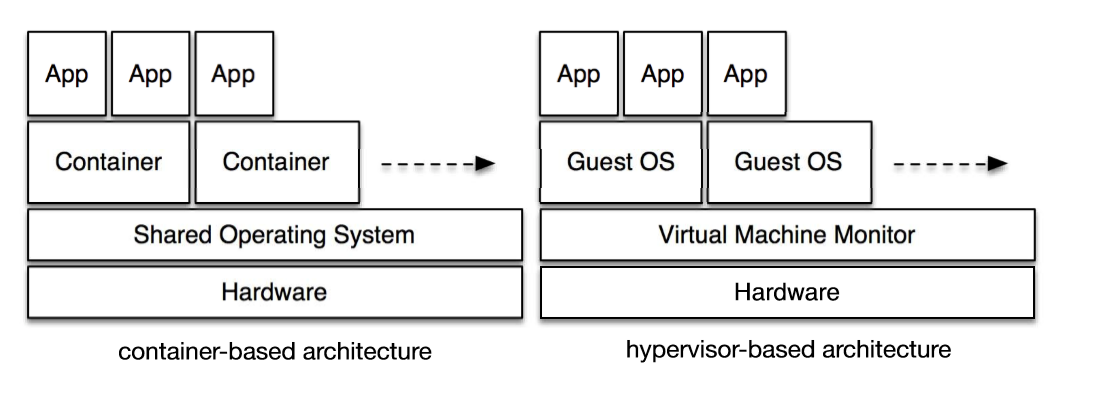
\includegraphics[width=1\linewidth]{pics/docker2.png}
	\captionof{figure}[Architektur Container und Virtuelle Maschine]{Architektur Container und Virtuelle Maschine \cite{Xavier2015AClouds}}
	\label{fig:architecture}
\end{minipage}

\subsubsection{Namespaces}
Dank der Einführung von Kernel-Namespaces ist es möglich, Ressourcen des Host-Systems wie CPU, Arbeitsspeicher, I/O und Netzwerk voneinander zu isolieren und diese unter bestimmten Voraussetzungen anderen Prozessen zur Verfügung zu stellen. 

Durch Namespaces werden die Ressourcen des Host-Systems in verschiedene Instanzen gepackt. Der innerhalb eines Namespaces gestartete Prozessaufruf sieht nur seine eigene Instanz und die unterliegende Baumstruktur seiner Kindprozesse. Der Prozess selbst hat die Illusion der vollständigen Ressourcenkontrolle über das komplette System, wobei diesem nur ein zugewiesener Teil zur Verfügung steht.

Aktuell existieren sieben verschiedene Namespaces. Diese sind \ac{PID}-Namespaces, Mount-Namespaces, \ac{UTS}-Namespaces, \ac{IPC}-Namespaces, Network-Namespaces, User-Namespaces und \ac{Cgroup}-Namespaces, die im Folgenden genauer erklärt werden.



\vspace{1em}
\begin{minipage}{\linewidth}
	\centering
	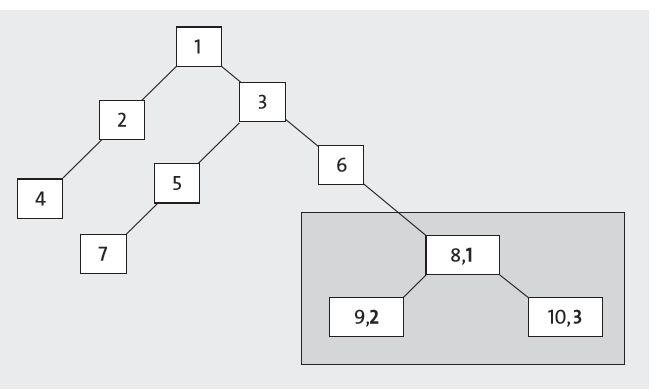
\includegraphics[width=1\linewidth]{pics/PID.PNG}
	\captionof{figure}[PID-Namespaces für Host und Container]{ PID-Namespaces für Host und Container (im Fettdruck) \cite{Liebel2017SkalierbareContainer-Infrastrukturen}}
	\label{fig:PID}
\end{minipage}

\subparagraph{PID-Namespaces} PID-Namespaces sind hierarchisch, deshalb kann ein Prozess nur die anderen Prozesse in seinem eigenen Namespace oder in seinen untergeordneten Namespaces sehen. Folglich kann der Host die Prozesse innerhalb des neuen PID-Namespace des Containers beobachten und beeinflussen. Die Prozesse innerhalb des Containers können die anderen Prozesse, die im Host oder in anderen Containern laufen, nicht beobachten oder beeinflussen. Die vereinfachte Darstellung des PID-Namespaces einer \emph{gespawnten} bzw. \emph{geforkten} Container-Prozess-Umgebung ist in Abbildung \ref{fig:PID} dargestellt. \cite{Liebel2017SkalierbareContainer-Infrastrukturen}

\subparagraph{Mount-Namespaces} Mount-Namespaces isolieren Filesystem Mountpunkte, die von einem Container gesehen werden. Somit können Prozesse in verschiedenen Containern unterschiedliche Ansichten der Filesystemhierarchie haben.

\subparagraph{UTS-Namespaces} UTS-Namespaces erlauben jedem Container seinen eigenen Hostnamen und \ac{NIS}-Domänennamen zu haben.

\subparagraph{IPC-Namespaces} IPC-Namespaces isolieren die Interprozesskommunikation. Das bedeutet, Prozesse die in einem Container enthalten sind, haben eigene Nachrichtenwarteschlangen und sind völlig unabhängig von Prozessen in anderen Containern.

\subparagraph{Network-Namespaces} Network-Namespaces isolieren das Netzwerk-Untersystem wie z.B. Geräte und IP-Adressen. Jeder Container unterhält seine eigene Netzwerkkonfiguration und die darauf laufenden Anwendungen.

\subparagraph{User-Namespaces} User-Namespaces isolieren Benutzer-IDs vom Host und anderen laufenden Containern. Das bedeutet, dass der Benutzer \emph{Root} (ID0) innerhalb eines Containers volle Privilegien hat, außerhalb jedoch keine Privilegien besitzt. Dies gewährleistet vor allem Sicherheit und Zuverlässigkeit \cite{Xavier2015AClouds}.

\subparagraph{Cgroup-Namespaces} Cgroup-Namespaces isolieren Cgroups untereinander, sodass keine Informationen über vorhandene Systemressourcen geteilt werden können.



\subsubsection{Cgroup}
\emph{Cgroup} steht für \ac{Cgroup}. Durch Cgroups ist es möglich, eine Reihe von Kriterien anzuwenden, um Ressourcen wie Speicher, Netzwerk, I/O und CPU einzuschränken. Ein Container sollte seine auferlegten Beschränkungen nicht überschreiten und andere Container, die auf derselben Hardware laufen, nicht stören. Cgroups sind für die Ressourcenbegrenzung, Priorisierung, Abrechnung und Kontrolle zuständig.

Durch Cgroups gibt es einen Weg, um Prozesse und Systemressourcen in einer kontrollierten und konfigurierbaren Weise hierarchisch zu organisieren. Cgroups bestehen im Wesentlichen aus zwei Teilen, dem Kern und dem Controller. Der Cgroup-Kern ist in erster Linie für die hierarchische Organisation von Prozessen zuständig. Der Cgroup-Controller ist in der Regel für die Verteilung einer bestimmten Art von Systemressource entlang der Hierarchie verantwortlich. Cgroups bilden eine Baumstruktur. Jeder Prozess im System gehört genau zu einer Cgroup. Alle Unterprozesse (Kindprozesse) eines Prozesses (Elternprozess) gehören zur gleichen Cgroup \cite{Heo2015ControlV2}. 


\paragraph{Ressourcenverteilungs-Modelle}
Cgroup-Controller verfügen über verschiedene Ressourcenverteilungs-Modelle. Diese Modelle sind auf die Art und den Verwendungszweck der Ressource zugeschnitten. Der folgende Paragraph befasst sich mit den verschiedenen Hauptschemen und deren Aufgaben \cite{Heo2015ControlV2}.

\subparagraph{Weight}
Beim Weight-Modell werden die zur Verfügung stehenden Ressourcen eines Prozesses proportional zur Gewichtung an alle aktiven Kindprozesse verteilt. Da nur die aktiven Kindprozesse, welche aktuell Ressourcen benötigen, an der Verteilung teilnehmen, sind die zugeteilten Ressourcen effizient genutzt. 

\subparagraph{Limit}
Das Limit-Modell bietet die Möglichkeit, verschieden Limits zu verwenden. Ist ein High-Limit gesetzt, kann ein Kindprozess die Ressource nur bis zu der konfigurierten Menge verwenden. Low/High-Limits können auch als Soft-Limits bezeichnet werden. Die Summe der Limits aller Kindprozesse kann die zur Verfügung stehende Menge an Ressourcen des Elternprozesses überschreiten. Ein Limit ist sozusagen ein maximaler Richtwert, der bei dringendem Bedarf überschritten werden kann. Der Prozess, welcher den über das Limit hinausragenden Anteil verwendet, steht unter erhöhtem Druck und wird gedrängt, die Ressource schnell wieder frei zu geben. Wenn eine Cgroup die Ressourcen nicht mehr benötigt, wird diese bis zu einem setzbaren Low-Limit freigegeben.


\subparagraph{Protection}
Im Protection-Modell ist eine Cgroup so geschützt, dass sie bis zur konfigurierten Menge der Ressource fest zugeordnet werden kann, solange die Verwendung aller Prozesse unter der geschützten Ebene liegt. Der Schutz kann garantiert oder effizient sein. Bei garantiertem Schutz wird die Ressource explizit für die Cgroup freigehalten und kann vollständig verwendet werden. Die effizientere Variante bietet die Möglichkeit, zugeteilte Ressourcen auf Anfrage für andere Prozesse freizustellen.


\subparagraph{Allocation}
Einer Cgroup wird eine bestimmte Menge einer Ressource fest zugeteilt und stellt somit ein Hard-Limit dar. Die Summe der Zuweisungen von Kindprozessen darf die Menge der fest zugeteilten Ressourcen des Elternprozesses nicht überschreiten. Auch wenn die Ressource nicht vollständig ausgenutzt wird, bleibt diese der Cgroup erhalten. 


\paragraph{Ressourcen-Modellierung}
Da nicht jede Hardwareressource auf die gleiche Art eingeschränkt werden kann, existieren Controller, die anhand der gerade beschriebenen Modelle, Ressourcen verwalten. Im folgenden Paragraphen werden die Art der Ressource mit den verwendeten Modellen genauer betrachtet, sowie unterschiedliche Varianten der Limitierung aufgezeigt. Besonderes Augenmerk ist auf die Speicherverwaltung gelegt.

\subparagraph{Speicher}
Der Speicher-Controller regelt die Verteilung des Speichers. Speicher ist zustandsabhängig und verwendet sowohl Limit- als auch Protection-Modelle. Aufgrund der Verflechtung zwischen Speicherbedarf und Speicherrückgabeforderung ist die Verwaltung sehr kompliziert.

\emph{Memory-Low (best-effort)}
Der geforderte Mindestanteil wird gestellt. Unbenutzter Speicher kann bei Bedarf vom System verwendet werden.

\emph{Memory-High (best-effort)}
Dies ist der Hauptmechanismus zur Steuerung des Speicherverbrauchs einer Cgroup. Wenn die Nutzung einer Cgroup über die obere Grenze hinausgeht, werden die Prozesse der Cgroup gedrosselt und unter starken Reklamationsdruck gesetzt.

\emph{Memory-Min (hard-limit)}
Falls der Speicherverbrauch einer Cgroup innerhalb seiner effektiven minimalen Grenze liegt, wird der Speicher der Cgroup unter keinen Umständen zurückgefordert. Wenn nicht genug Speicherplatz zur Verfügung steht um die Minimalanforderung zu gewährleisten, kommt der OOM-Killer (siehe Kapitel \ref{Isolation Container}) zum Einsatz und schafft freien Speicher.

\emph{Memory-Max (hard-limit)}
Wenn der Speicherverbrauch einer Cgroup diese gesetzte Grenze erreicht und nicht reduziert werden kann, wird der OOM-Killer in der Cgroup aufgerufen. Dies ist der letzte Schutzmechanismus. Unter bestimmten Umständen kann ein Prozess vorübergehend über das Limit hinaus gehen.

\subparagraph{CPU}
Der CPU-Controller reguliert die Verteilung der CPU-Zyklen. Diese Steuerung verwendet Weight- und Limit-Modelle für normale Ressourcenverteilung und das Allocation-Modell für eine Echtzeitverteilung.

\subparagraph{I/O}
Der I/O-Controller reguliert die Verteilung der I/O-Ressourcen. Der Controller verwendet Weight- und Limit-Modelle. Die Gewichtung gibt die relative I/O-Zeit an, welche die Cgroup in Bezug auf ihre Geschwister verwenden kann.

\subsection{Hypervisor-basierte Virtualisierung}
Eine \ac{VM} bildet mit Hilfe des \emph{Hypervisors}, auch \ac{VMM} genannt, eine komplette Rechnerarchitektur auf dem Host-Rechner ab (siehe Abbildung \ref{fig:architecture}). Der Hypervisor ist ein modifizierter minimaler Betriebssystem-Kernel. Man unterscheidet zwischen zwei Arten von VMM: Dem Typ-1-VMM oder \emph{bare-metal-hypervisor}, welcher direkt auf der zugrundeliegenden Hardware des Hosts liegt und dem Typ-2-VMM \emph{hostet-hypervisor}, der eine komplette virtuelle Maschine auf dem Host-Betriebssystem erstellt. Die Grundanforderung eines VMM sind nach Popek/Goldberg \cite{Popek1974FormalArchitectures,Glatz2015Betriebssysteme}:


 \subparagraph{Equivalence} 
 Prozesse, die auf der virtuellen Maschine gestartet werden, laufen wie Prozesse auf dem  Host-System identisch ab, mit Ausnahme der Geschwindigkeit. 
 
\subparagraph{Efficiency} 
Alle unkritischen Prozesse werden von der Hardware direkt ausgeführt, ohne Eingreifen des VMM.

\subparagraph{Resource control} 
Es darf kein Prozess Ressourcen verwalten. Bei jedem Zugriffsversuch eines Prozesses auf Systemressourcen wird der VMM aufgerufen.



\subsubsection{Typ-1-VMM}
Der bare-metal-hypervisor, schematisch dargestellt in Abbildung \ref{fig:Hypervisor_Typ1/Typ2} a, liegt direkt auf der Hardware und hat uneingeschränkten Zugriff darauf. Der VMM kümmert sich um die Ressourcenverwaltung und die isolierte Bereitstellung von virtuellen Maschinen. Die Aufteilung der Rechenzeit (CPU) und die Zuteilung von Speicher auf die einzelnen VMs sind Beispiele der Aufgaben, welche die Ressourcenverwaltung beinhaltet. Dieser Virtualisierungsansatz wird beispielsweise von \emph{Xen} \cite{Install2018XenArchitecture} verwendet,  der nur mit einem eigenen, auf die Hardware zugeschnittenen Treiber, laufen kann \cite{Glatz2015Betriebssysteme}.

\vspace{1em}
\begin{minipage}{\linewidth}
	\centering
	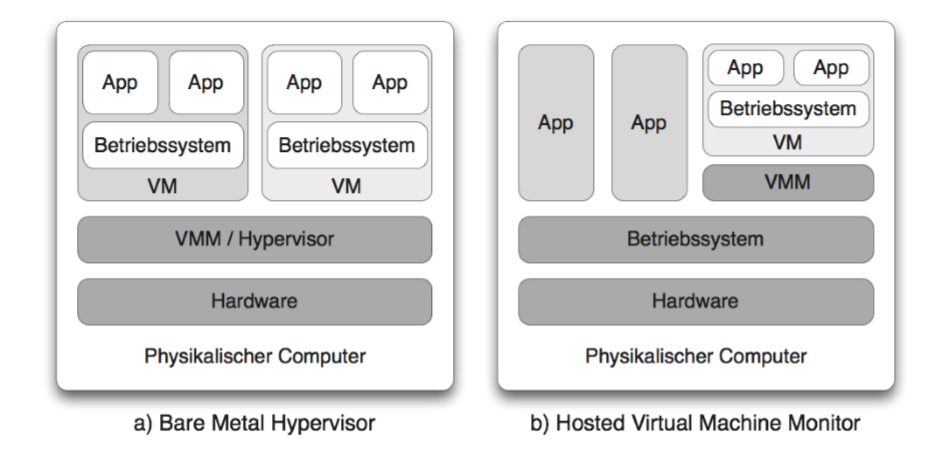
\includegraphics[width=1\linewidth]{pics/Hypervisoren.PNG}
	\captionof{figure}[Hypervisor Typ1/Type2]{Hypervisor Typ1-/Typ-2 \cite{Meinel2011VirtualisierungMarktubersicht} }
	\label{fig:Hypervisor_Typ1/Typ2}
\end{minipage}

\subsubsection{Typ-2-VMM}
Ein gehosteter Hypervisor teilt sich ein Host-Betriebssystem mit anderen Applikationen (siehe Abbildung \ref{fig:Hypervisor_Typ1/Typ2} b). Um die nötigen Rechte auf der Hardware zu erhalten, wird ein spezieller VMM-Treiber verwendet, der direkt unter dem Host-System installiert wird. Dieser ermöglicht privilegierten Zugriff auf die Hardware. \emph{VMware Workstation} ist ein Produkt dieser Realisierung der Virtualisierung \cite{Glatz2015Betriebssysteme}.

\subsubsection{Hybridformen}
Hypervisor die von Haus aus direkt in das Betriebssystem integriert wurden, sind zwischen Typ-1 und Typ-2 anzusiedeln. Die Realisierung von Linux heißt \ac{KVM}, das Pendant von Windows ist \emph{Hyper-V}. Diese Hybridformen sind die aktuell performantesten Hypervisor. 

\subsubsection{Hypervisor Virtualisierungsformen}
 Ressourcenanfragen, die das Gastsystem an die CPU sendet, müssen von der Virtualisierungsschicht (Hypervisor) abgefangen und interpretiert werden \cite{Meinel2011VirtualisierungMarktubersicht}. Das geschieht entweder über vollständige, Para- oder hardwareunterstütze Virtualisierung.  Es gibt bei aktuellen Prozessoren eine Rechteverwaltung, welche als Ringdiagramm darstellbar ist, siehe Abbildung \ref{fig:Ringmodell1}. Im Ring 0 besitzt man volle Zugriffsrechte auf Hardwareressourcen. Auf dieser Ebene ist der Kernel beheimatet. Die Ringe 1 und 2 stehen für Treiber zur Verfügung und in Ring 3, der die eingeschränktesten Zugriffsrechte enthält, sind alle sonstigen Anwendungen beheimatet. Die Kernel der Gastbetriebssysteme befinden sich grundsätzlich ebenfalls in dem 3. Ring. Im Folgenden wird genauer auf die drei eben erwähnten Virtualisierungsmethoden eingegangen. Eine Zusammenstellung der Virtualisierungmethoden ist in Abbildung \ref{fig:Virtualisierungen_Hypervisor} dargestellt.

\subparagraph{Vollständige Virtualisierung}
 Wenn eine Anwendung mit einem \emph{Systemcall} direkt auf einen vom Host-Kernel reservierten Speicherbereich zugreifen will, tritt eine Speicherschutzverletzung auf. Der Zugriff wird verweigert, was den Prozess abstürzen lässt. Der Hypervisor fängt solche kritischen Anfragen ab, überprüft diese, codiert die Anfragenstellung gegebenenfalls um und führt sie selbst mit höheren Zugriffsrechten aus. Nach dem Aufruf folgt eine entsprechende Rückübersetzung und Rückgabe an die aufrufende virtuelle Maschine. Diesen Vorgang nennt man \emph{binary translation}, der sehr häufig durchgeführt werden muss. Dies führt zu einem erheblichen Overhead, der signifikante Leistungseinbußen zur Folge hat \cite{Meinel2011VirtualisierungMarktubersicht}. 
 
 \vspace{1em}
\begin{minipage}{\linewidth}
	\centering
	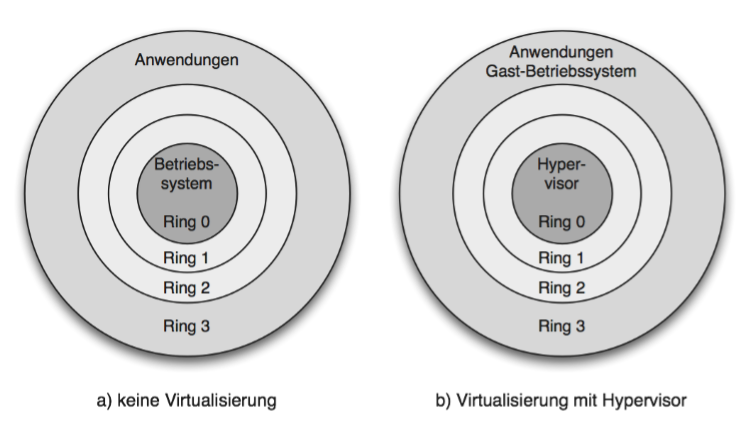
\includegraphics[width=1\linewidth]{pics/Ringmodell1.PNG}
	\captionof{figure}[Ringdiagramm Zugriffsverwaltung ]{Ringdiagramm Zugriffsverwaltung \cite{Meinel2011VirtualisierungMarktubersicht} }
	\label{fig:Ringmodell1}
\end{minipage}
 
 \subparagraph{Para-Virtualisierung}
 Bei der Para-Virtualisierung werden die Kernel der Gastbetriebssysteme so angepasst, dass diese auf Ring 1 laufen können. Was vorher \emph{Systemcalls} waren und vom Betriebssystem verweigert wurden, sind jetzt \emph{Hypercalls}, die direkt an den Hypervisor gesendet werden. Der Hypervisor führt den entsprechenden Systemaufruf aus und bedient die aufrufende virtuelle Maschine \cite{Meinel2011VirtualisierungMarktubersicht}. Um diese effizientere Methode der Virtualisierung zu verwenden, ist eine darauf zugeschnittene Hardware nötig.

\vspace{1em}
\begin{minipage}{\linewidth}
	\centering
	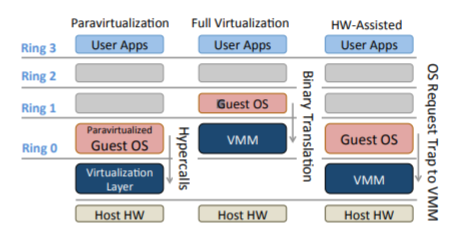
\includegraphics[width=0.8\linewidth]{pics/Virtualisierungen_Hypervisor.PNG}
	\captionof{figure}[Virtualisierungen Hypervisor]{Virtualisierungen Hypervisor \cite{Fayyad-Kazan2013BenchmarkingHypervisors}}
	\label{fig:Virtualisierungen_Hypervisor}
\end{minipage}
 
\subparagraph{Hardwareunterstützte Virtualisierung}
Durch die Hardwareunterstützung von \emph{Intel VT-x} \cite{TechnologyIntel} oder \emph{AMD-v} \cite{AMDVirtualisierungstechnologie}, die den Prozessor-Befehlssatz erweitern, können virtuelle Maschinen \emph{Systemcalls} nativ ausführen. Somit müssen die Kerne der Gastbetriebssysteme nicht modifiziert werden, wie es bei der Para-Virtualisierung gemacht wird. Die hardwareunterstützte Variante ist die performanteste Methode der Hypervisor-Technologien \cite{Meinel2011VirtualisierungMarktubersicht}.




%\pagebreak
